% Chapter Template

\chapter{Experiments} % Main chapter title

\label{Chapter3} % Change X to a consecutive number; for referencing this chapter elsewhere, use \ref{ChapterX}

\lhead{Chapter 3. \emph{Experiments}} % Change X to a consecutive number; this is for the header on each page - perhaps a shortened title

%----------------------------------------------------------------------------------------
%	SECTION 1
%----------------------------------------------------------------------------------------

\section{Experimental Setup}

To simulate a fat-tree topology as seen in data center networks, 4 physical servers and 2 data plane programmable switches were used. Each switch
was virtualized to create 5 switches using 10G loopback links. So, we have 10 switches in total, with 4 of them as top-of-rack or edge switches,
4 of them as aggregate switches, and 2 as core switches (Figure \ref{fig:Topology})

\begin{figure}[htbp]
	\centering
		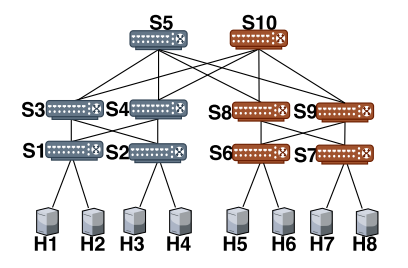
\includegraphics[width=0.65\columnwidth]{Figures/Topology.png}
		\rule{35em}{0.5pt}
	\caption[Evaluation Topology]{Evaluation Topology}
	\label{fig:Topology}
\end{figure}
\clearpage
The rest of this chapter is structured as follows: For a potential fault that can occur in the network, we have
\begin{itemize}
    \item A section on the description of the fault
    \item A section on the configuration of switches and hosts for reproducing the fault
    \item A section on how the proposed fault can be diagnosed using SQL queries
    \item Results and relevant illustrations
\end{itemize}

The last section presents a unified scheme for diagnosing faults in network built on logic that has been developed
in preceding sections.

\section{The Synchronous Incast Problem}
\subsection{Description}
\subsection{Configuration}
\subsection{Diagnosis}
\subsection{Results and Illustrations}

\section{Asynchronous Incast problem and Heavy Hitters}
\subsection{Description}
\subsection{Configuration}
\subsection{Diagnosis}
\subsection{Results and Illustrations}

\section{Link Underprovisioning}
\subsection{Description}
\subsection{Configuration}
\subsection{Diagnosis}
\subsection{Results and Illustrations}

\section{A unified sceme}